% !TEX root =  manual.tex

\section{Covariance Functions Recognized by the Emulator}
\label{sec:CovarianceFunctions}

$u$ and $v$ are zero-indexed vectors that represent a point in parameter space.  $P$ is the number of parameters. $\Theta=(\theta_0, \theta_1,\theta_2,\ldots)$ is a list of $P+2$ or $P+3$ hyperparameters. $\theta_0$ is called \emph{amplitude}; $\theta_1$ is called the \emph{nugget}.  $\Vert\,\cdotp\Vert{}_\Theta$ is a distance function parametrized by $\Theta$.  $\epsilon$ is $10^{-5}$. $c_\Theta{}(u, v)$ is the covariance between $u$ and $v$, as parametrized by $\Theta$.


\begin{figure}[b]
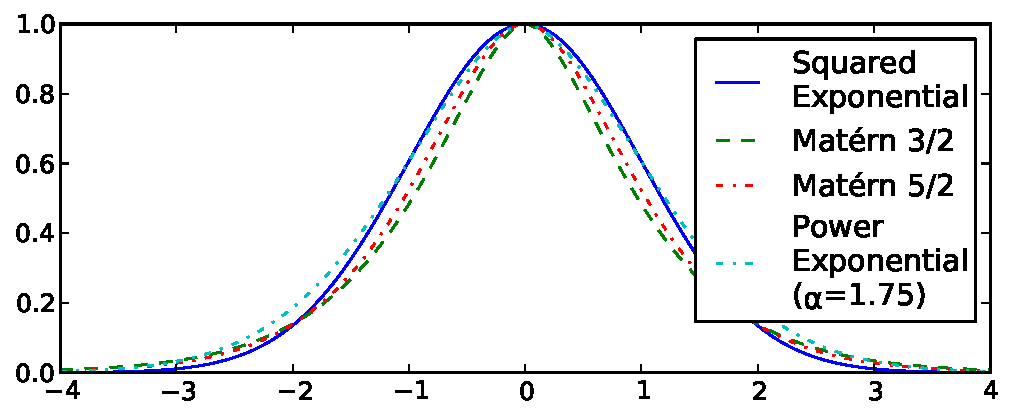
\includegraphics[width=4in]{figs/kernel_functions.pdf}
\parbox[b]{2.5in}
{\caption{\label{fig:kernelfunctions}
$C_\Theta{}(0, x)$ for a one-dimensional parameter space with each covariance function type. The amplitude is 1, the nugget is 0, and the length scale is 1.
\vspace*{30pt}
}}
\end{figure}

%% FIGURE SOURCE CODE:
%%
%% #!/usr/bin/env python
%% import matplotlib.pyplot
%% import numpy
%% x = numpy.arange(-4,4,0.01)
%% SE = numpy.exp(-0.5 * (x ** 2))
%% alpha = 1.75
%% PE = numpy.exp(-0.5 * (numpy.power(numpy.abs(x),alpha)))
%% M52 = (1 + numpy.sqrt(5) * numpy.abs(x) + 5/3.0 * (
%%     (numpy.abs(x))**2) ) * numpy.exp(- numpy.sqrt(5) *
%%     numpy.abs(x))
%% M32 = (1 + numpy.sqrt(3) * numpy.abs(x) ) * numpy.exp(
%%     - numpy.sqrt(3) * numpy.abs(x))
%% matplotlib.pyplot.plot(x, SE,  '-',  label=u'Squared\nExponential')
%% matplotlib.pyplot.plot(x, M32, '--', label=u'Mat\u00e9rn 3/2')
%% matplotlib.pyplot.plot(x, M52, '-.', label=u'Mat\u00e9rn 5/2')
%% matplotlib.pyplot.plot(x, PE, ':',
%%     label=u'Power\nExponential\n(\u03b1=%g)'%alpha)
%% matplotlib.pyplot.legend()
%% matplotlib.pyplot.axes().set_aspect(3)
%% matplotlib.pyplot.savefig('kernel_functions.pdf',
%%     bbox_inches='tight')


\begin{itemize}
\item Squared-Exponential [\variable{SQUARE\_EXPONENTIAL\_FUNCTION}]
\[ \Vert{}u-v\Vert{}_\Theta{} = \sqrt{\sum_{i=0}^{P-1} \frac{(u_i - v_i)^2}{(\theta{}_{2+i})^2}} \qquad
 \delta{}_{uv} = 1 \text{ if } (\Vert{}u-v\Vert{}_\Theta{} < \epsilon{}) \textrm{ else } \delta{}_{uv} = 0 \]
\[ c_\Theta{}(u, v) = \theta{}_0 \exp\left({-\tfrac{1}{2} \Vert{}u-v\Vert{}_\Theta{}^2}\right) + \theta{}_1\delta{}_{uv} \]

\item {Power-Exponential}
[\variable{POWER\_EXPONENTIAL\_FUNCTION}]
\[ \Vert{}u-v\Vert{}_\Theta{} = \sqrt{\sum_{i=0}^{P-1} \frac{(u_i - v_i)^2}{(\theta{}_{3+i})^2}} \qquad
 \delta{}_{uv} = 1 \text{ if } (\Vert{}u-v\Vert{}_\Theta{} < \epsilon{}) \textrm{ else } \delta{}_{uv} = 0 \]
\[ c_\Theta{}(u, v) = \theta{}_0 \exp\left({-\tfrac{1}{2} \Vert{}u-v\Vert{}_\Theta{}^{\theta{}_2}}\right) + \theta{}_1\delta{}_{uv} \]

\item {Mat\'{e}rn 3/2}
[\variable{MATERN\_32\_FUNCTION}]
\[ \Vert{}u-v\Vert{}_\Theta{} = \sqrt{\sum_{i=0}^{P-1} \frac{(u_i - v_i)^2}{(\theta{}_{2+i})^2}} \qquad
 \delta{}_{uv} = 1 \text{ if } (\Vert{}u-v\Vert{}_\Theta{} < \epsilon{}) \textrm{ else } \delta{}_{uv} = 0 \]
\[ c_\Theta{}(u, v) = {\theta{}_0} \left({ 1 + \sqrt{3} \Vert{}u-v\Vert{}_\Theta{} }\right)
\exp \left({ - \sqrt{3} \Vert{}u-v\Vert{}_\Theta{} }\right) + \theta{}_1\delta{}_{uv} \]


\item {Mat\'{e}rn 5/2}
[\variable{MATERN\_52\_FUNCTION}]
\[ \Vert{}u-v\Vert{}_\Theta{} = \sqrt{\sum_{i=0}^{P-1} \frac{(u_i - v_i)^2}{(\theta{}_{2+i})^2}} \qquad
 \delta{}_{uv} = 1 \text{ if } (\Vert{}u-v\Vert{}_\Theta{} < \epsilon{}) \textrm{ else } \delta{}_{uv} = 0 \]
\[ c_\Theta{}(u, v) = {\theta{}_0} \left({ 1 + \sqrt{5} \Vert{}u-v\Vert{}_\Theta{}
 + \tfrac{5}{3} \left({\Vert{}u-v\Vert{}_\Theta{}}\right)^2  }\right) + \theta{}_1\delta{}_{uv} \]
\end{itemize}

%%  LocalWords:  hyperparameters
